%%%%%%%%%%%%%%%%%%%%%%%%%%%%%%%%%%%%%%%%%%%%%%%%%%%%%%%%%%%%%%

\documentclass[12pt,ITBthesis]{report}

\usepackage{amsfonts}
\usepackage{amssymb,amsmath}
\usepackage{amsthm}
\usepackage{newlfont}
\usepackage{graphicx}
\usepackage{tabularx}
\usepackage{longtable}
\usepackage{lscape}
%\usepackage{rotating}
\usepackage{latexsym}
\usepackage{natbib}
\usepackage{geometry}
\usepackage{fancyhdr}
\usepackage{xthesis}
\usepackage{xtocinc} %Include Table of Contents as the first entry in TOC
\usepackage{subfigure}
\usepackage{times}
\usepackage[hidelinks]{hyperref}



\bibpunct[, ]{(}{)}{;}{a}{,}{,}


\begin{document}
% \begin{KeepFromToc}
%   \tableofcontents
% \end{KeepFromToc}


%%% this section is responsible for creating bookmarks and cross-links in your pdf document
%\hypersetup{bookmarksnumbered=true, colorlinks=false, bookmarksopen = false, linkcolor=blue ,
%linkbordercolor = 3 3 3, citebordercolor = 3 3 3, urlbordercolor = 3 3 3}


% Fuzz -------------------------------------------------------------------
\hfuzz2pt % Don't bother to report over-full boxes if over-edge is < 2pt
% Line spacing -----------------------------------------------------------

\newlength{\defbaselineskip}
\setlength{\defbaselineskip}{\baselineskip}
\newcommand{\setlinespacing}[1]%
           {\setlength{\baselineskip}{#1 \defbaselineskip}}
\newcommand{\doublespacing}{\setlength{\baselineskip}%
                           {2.0 \defbaselineskip}}
\newcommand{\singlespacing}{\setlength{\baselineskip}{\defbaselineskip}}
% MATH -------------------------------------------------------------------
\newcommand{\A}{{\cal A}}
\newcommand{\h}{{\cal H}}
\newcommand{\s}{{\cal S}}
\newcommand{\W}{{\cal W}}
\newcommand{\BH}{\mathbf B(\cal H)}
\newcommand{\KH}{\cal  K(\cal H)}
\newcommand{\Real}{\mathbb R}
\newcommand{\Complex}{\mathbb C}
\newcommand{\Field}{\mathbb F}
\newcommand{\RPlus}{[0,\infty)}
%
\newcommand{\norm}[1]{\left\Vert#1\right\Vert}
\newcommand{\essnorm}[1]{\norm{#1}_{\text{\rm\normalshape ess}}}
\newcommand{\abs}[1]{\left\vert#1\right\vert}
\newcommand{\set}[1]{\left\{#1\right\}}
\newcommand{\seq}[1]{\left<#1\right>}
\newcommand{\eps}{\varepsilon}
\newcommand{\To}{\longrightarrow}
\newcommand{\RE}{\operatorname{Re}}
\newcommand{\IM}{\operatorname{Im}}
\newcommand{\Poly}{{\cal{P}}(E)}
\newcommand{\EssD}{{\cal{D}}}
% THEOREMS ---------------------------------------------------------------
\theoremstyle{plain}
\newtheorem{thm}{Theorem}[section]

\newtheorem{cor}[thm]{Corollary}
\newtheorem{lem}[thm]{Lemma}
\newtheorem{prop}[thm]{Proposition}
%
\theoremstyle{definition}
\newtheorem{defn}{Definition}[section]
%
\theoremstyle{remark}
\newtheorem{rem}{Remark}[section]
%
\numberwithin{equation}{section}
\renewcommand{\theequation}{\thesection.\arabic{equation}}
%%% ----------------------------------------------------------------------
\setlength{\tclineskip}{1.05\baselineskip}
%%% ----------------------------------------------------------------------

\makeatletter
\renewcommand\listoffigures{%
        \@starttoc{lot}%
}
\makeatother

\makeatletter
\renewcommand\listoftables{%
        \@starttoc{lot}%
}
\makeatother

\makeatletter
\renewcommand\appendix{%
 \par
 \setcounter{chapter}{0}%
 \setcounter{section}{0}%
 \setcounter{subsection}{0}%
 \gdef\thesection{\@Alph\c@section}
 \gdef\@sect##1##2##3##4##5##6[##7]##8{%
  \refstepcounter{##1}%
  \protected@edef\@svsec{\@seccntformat{##1}\relax}%
  \begingroup
    \hspace{-\parindent}##6\appendixname~ {%
    \@hangfrom{\hskip ##3 \relax\@svsec}\par%
    \hspace{-\parindent}\interlinepenalty \@M ##8 \@@par}%
  \endgroup
  \csname ##1mark\endcsname{##7}%
  \addcontentsline{toc}{##1}{\protect\numberline{\csname the##1\endcsname}##7}%
  \@xsect{##5}%
 }%
}%
\makeatother

\setlength{\parskip}{1ex plus 0.5ex minus 0.2ex}


\title{Thesis Proposal\\ TITLE HERE}

\author{NAME HERE}

\university{Institute of Technology Blanchardstown }

\dept{School of Informatics and Engineering }

\address{Dublin, Ireland }

\supervisor{}

\submitdate{2017}

\degree{B.Sc in Computing and Information Technology}


%\dedicate{To my wife\\
% \begin{Huge}{\textbf{Glenda}}\end{Huge}}

%\nobib
%\draft
%\nofront
%\permissionfalse
%\include{ABS}

\setcounter{page}{1} \beforepreface



{ \typeout{Abbreviations}
% Thesis Abbreviation ------------------------------------------------------

\prefacesection{Abbreviations}


%%%%%%%%%%%%%%%%%%%%%%%%%%%%%%%%%%%%%%%%%%%%%%%%%%%%%%%%%%%%%%%%%%%%%%%%%%%%%%%%
% Create a list of all abbreviations that you've used throughout your thesis.  %
% Order the abbreviations in alphabetical order                                %
%%%%%%%%%%%%%%%%%%%%%%%%%%%%%%%%%%%%%%%%%%%%%%%%%%%%%%%%%%%%%%%%%%%%%%%%%%%%%%%%

\begin{longtable}{p{90pt}l}
\hline ANN    	&\vline  Artificial Neural Network \\
\hline CNN      &\vline  Convultional Neural Network \\
\hline ReLU     &\vline  Rectified Linear Unit \\
\hline 
\
\end{longtable}






% ----------------------------------------------------------------------
 %write your list of abbreviations in a file called abbreviations.tex
}

%{ \typeout{Glossary}
%\include{glossary}
%}



% ------------------------------------------------------------------------
\afterpreface
\def\baselinestretch{1}
\setlinespacing{1.66}
% ------------------------------------------------------------------------

\pagestyle{fancy}
% \renewcommand{\chaptermark}[1]% 
%{\markboth{\MakeUppercase{\thechapter.\ #1}}{}}
% \renewcommand{\sectionmark}[1]%
%{\markright{\MakeUppercase{\thesection.\ #1}}}
\renewcommand{\headrulewidth}{0.5pt}
\renewcommand{\footrulewidth}{0pt}
\newcommand{\helv}
{%
\fontfamily{bch}\fontseries{b}\fontsize{9}{11}\selectfont} \fancyhf{} \fancyhead[LE,RO]{\helv \thepage}
\fancyhead[LO]{\helv \rightmark} \fancyhead[RE]{\helv \leftmark}

% ------------------------------------------------------------------------
\setlinespacing{1.0}

\prefacesection{Text Analytics Using Rapid Miner}

\section*{Business Understanding}

This following sections shall describe the business objectives, the mining objectives, a analysis and plan for the proposed project.

\subsection*{Business Objective}
The objective of this project is to mine unstructured data using Rapid Miner.

\subsection*{Data Mining objective}
\begin{itemize}
	\item The main objective is to mine articles about Machine Learning, Deep Learning and Robotics. 
	\item Web crawling will be implemented to find related text on the topics.
	\item Preprocessing steps shall be put in place in order to produce the most predictive words for modeling.
	\item Multiple clustering and classification models will be used to identify the texts.
\end{itemize}

\subsection*{Project analysis}
% (cost benifit analysis; risk assessment; resouces needed; assumptions)
In terms of a cost benefit analysis, this project deems relatively efficient due to the benefits out weighing the costs. The proposed assignment poses minimal risk as only a few events may delay the production of the project, such as unavailable texts and misclassification, which are very unlikely. The resources required for this project include: The RapidMiner software and all it's operators related to the data mining objective, articles from online resources, 13 documents based on 3 categories and a online word cloud service for visualisation of predictive words or phrases. 

 
\subsection*{Project plan}
There are a number of steps taken in relation to this project.
\begin{itemize}
	\item Initially, Three categories are decided on. Two topics should be relatively similar, and the last on will be unrelated. In this case, they are based on Deep Learning, Machine Learning and robitics.
	\item Thirteen texts are sourced online for each category. Ten shall be used for training datasets and three shall be used for testing. Web crawling will be implemented using RapidMiner for three of those texts. The steps taken will be documented 
	\item These source articles will be downloaded into their respective folders based on their class label.
	\item A word cloud will be creating to visualise the frequently occurring terms.
	\item Preprocessing steps shall be experimented with to compare stemmers, determine which words are predominantly more predictive, apply pruning and comparing accuracy based on different vectors and documenting the results.
	\item Apply two algorithms for clustering and classification and discuss the accuracy of them.
	\item Lastly, an evaluation of the project will be performed, which will assess the overall result in relation with the business objectives. 
\end{itemize}

%%%%%%%%%%%%%%%%%%%%%%%%%%%%%%%%%%%%%%%%%%%%%%%%%%%%%%%%%%%%

\section*{Data Understanding}
%Eliminate common words & stop words
%Eliminate rare words
%Identify phrases

As previously mentioned, thirteen texts have been obtain online according to three categories: machine learning, deep learning and robotics.
In order to obtain a better insight to the commonly occurring word in the files of each category, word clouds were made. As seen in Figure \ref{mlfig}, Figure \ref{dlfig} and Figure \ref{robfig} three word images were made to visualise the frequent terms. The larger the word appears in the image, the more often it appears in the documents that have been collected.
For machine learning, it is clear that the terms \textbf{knn}, \textbf{training}, \textbf{decision tree}, \textbf{naive bayes} and \textbf{classification}.

\begin{figure}[ht]
	\begin{center}
		\advance\leftskip-3cm
		\advance\rightskip-3cm
		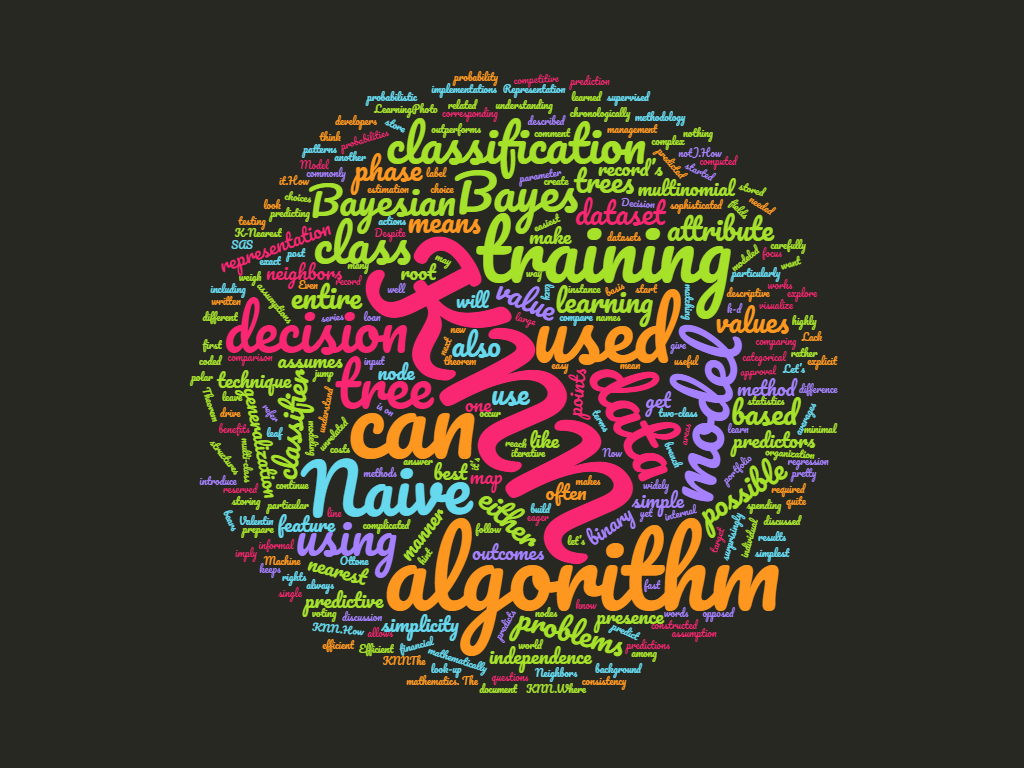
\includegraphics[keepaspectratio=true,scale=0.4]{__resources/machine_learning.png}
		\caption{Word cloud for the machine learning category}
		\label{mlfig}
	\end{center}
\end{figure}

\newpage

A more concise description of deep learning can be seen in Figure 2. Although the two categories are related, these terms seem to focus more so on words like \textbf{networks}, \textbf{neural}, \textbf{CNN's}, \textbf{model} and \textbf{recurrent} to name a few.

\begin{figure}[ht]
	\begin{center}
		\advance\leftskip-3cm
		\advance\rightskip-3cm
		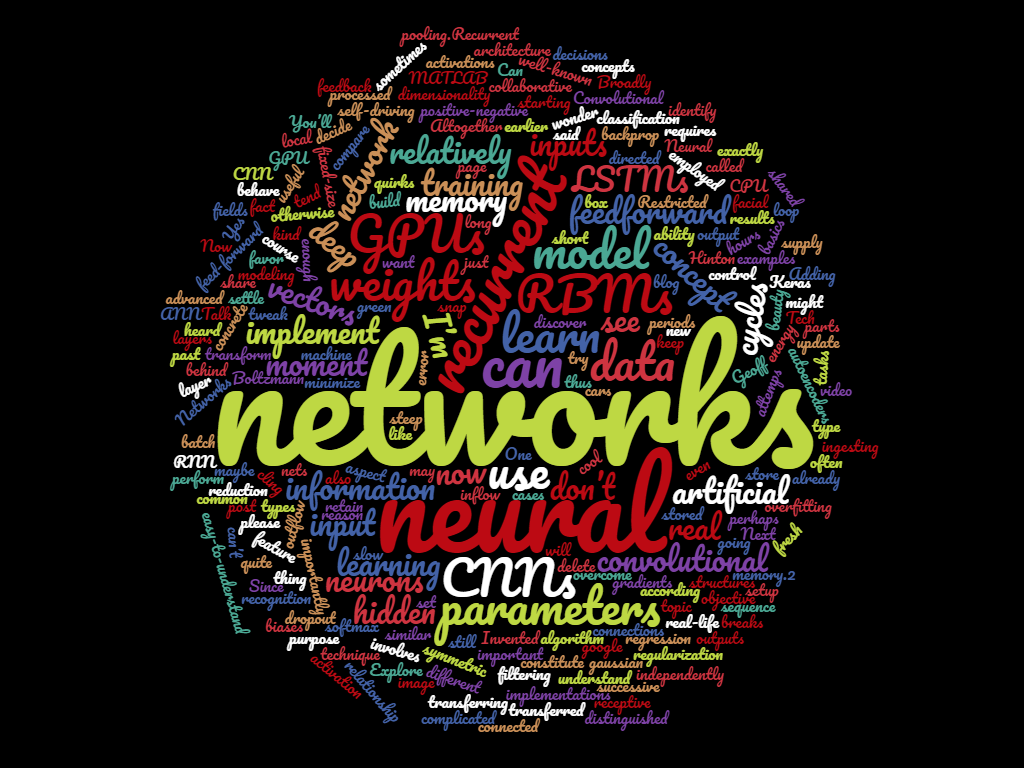
\includegraphics[keepaspectratio=true,scale=0.4]{__resources/deep_learning.png}
		\caption{Word cloud for the deep learning category}
		\label{dlfig}
	\end{center}
\end{figure}

Lastly, we see the terms generated for the robotics category. Evidently, these words are not related to machine learning or deep learning as they share very few words to the documents in the other two categories. The prominent words found here are \textbf{robots}, \textbf{humans} or \textbf{humanoid} and  \textbf{robotics}

\newpage


\begin{figure}[ht]
	\begin{center}
		\advance\leftskip-3cm
		\advance\rightskip-3cm
		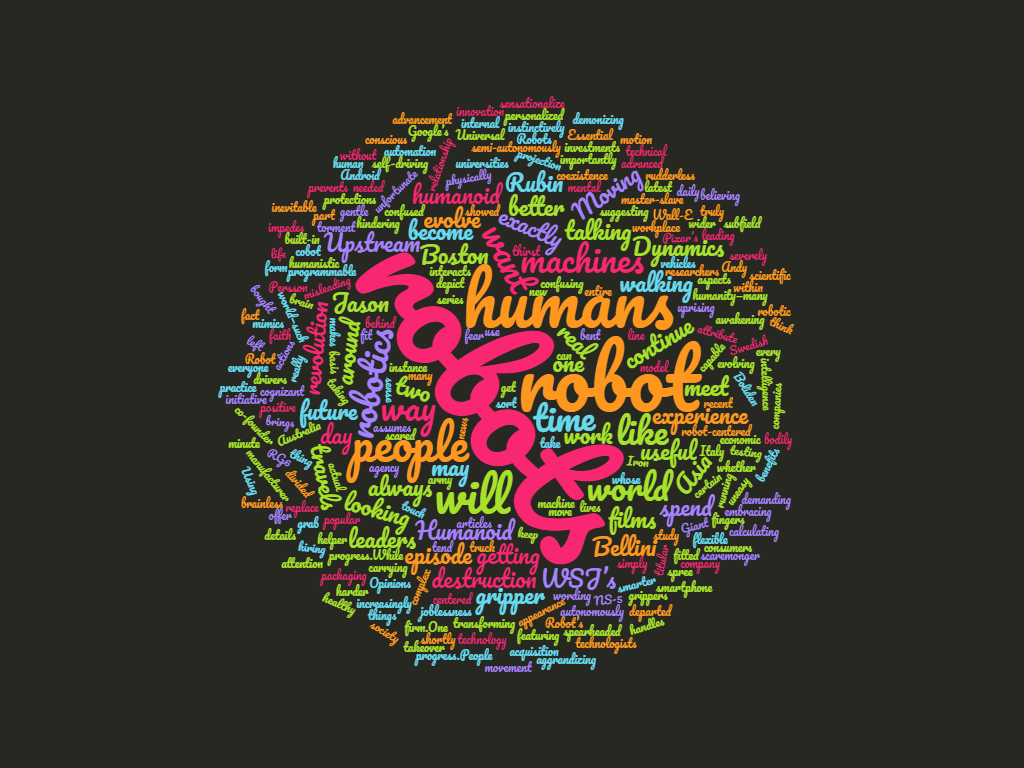
\includegraphics[keepaspectratio=true,scale=0.4]{__resources/robotics.png}
		\caption{Word cloud for the robotics category}
		\label{robfig}
	\end{center}
\end{figure}


Not only do these word clouds help determine predictive words, but also provide certain words that are not useful for the mining objects,also known as stop words. Certain stop words in these figures are "I'm", "thing",  "makes" for example. These words can be ambiguous depending on the sentiment of the article being read or just common English phrases, therefore they should not be included in the working model. \\
Furthermore, potential synonyms can be found in these word clouds. To reduce dimensionality, it is beneficial to specify words that may hold the same meaning. For instance, it can be seen that in the category of robotics, the terms "robot" and "robotics" are in interchangeable, therefore they can be classes as synonyms of one another. Another example of this could be the phase "neural network" and "ANN", which the latter is a acronym for "neural network" therefore that can also be classed as a synonym.

\newpage

%%%%%%%%%%%%%%%%%%%%%%%%%%%%%%%%%%%%%%%%%%%%%%%%%%%%%%%%%%%%
\newpage
\section*{Data Preparation}



%Generate a document vector based on
%selected concepts (terms and phrases)


%%%%%%%%%%%%%%%%%%%%%%%%%%%%%%%%%%%%%%%%%%%%%%%%%%%%%%%%%%%%
\section*{Modeling}

\subsection*{Modeling techniques}
\subsubsection*{Clustering}

\subsubsection*{Classification}

\subsection*{Test Design}
%e.g. split documents into training set and test set

\subsection*{Build and Assess the Model}

%%%%%%%%%%%%%%%%%%%%%%%%%%%%%%%%%%%%%%%%%%%%%%%%%%%%%%%%%%%%

\section*{Evaluation}
%Assessment of data mining reults with
%respect to original business objectives

%%%%%%%%%%%%%%%%%%%%%%%%%%%%%%%%%%%%%%%%%%%%%%%%%%%%%%%%%%%%
\subsection*{Project review}

\subsection*{Project deployment}
%Generate document vectors for new
%documents, and run the model.



\prefacesection{Assignment}


The initial steps of implementing a fuzzy logic system are as follows:
\begin{itemize}
	\item Crisp inputs are converted to set of fuzzy linguistic variable, linguistic terms and membership functions in what is known as fuzzification. 
	\item Based on a set of rules, an inference is made
	\item Lastly, defuzzification is implemented by using the membership functions to provide crisp results.
\end{itemize}
Linguistic variables are natural language values assigned to ranges of numeric inputs or outputs. These linguistic variables can have a set of real life terms to used to define a portion of the overall variable. For example, the linguistic variable \textbf{height} may have the terms {short, medium or tall etc.}. 

\section*{Linguistic Variables}
Based on the requirements of the system, linguistic variables need to be defined for the fuzzy logic system. We know that there are two input variables: "Level" and "Demand". Additionally, an output variable is specified to represent the command given to the pumping system, which will be defuzzified to a final crisp output. Each of these variables should be segmented into the appropriate terms. 
\subsection*{Level}
With this variable, five terms have been used to define the ranges of the level in the water. The terms are as follows: 
\textbf{Level(l) = {very\_low, low, average, high, very\_high}.}\\
The membership functions are based on the ranges specified in the assignment document. Level of the water in the tank can range from between 0 and 100. The type of membership functions used are trapezoidal and triangle. The trapezoidal function are used on the most extreme cases such as very\_low and very\_high and triangle are used on the low, average and high. See figure \ref{member1} for graphical representation.

\begin{figure}[ht]
	\begin{center}
		\advance\leftskip-3cm
		\advance\rightskip-3cm
		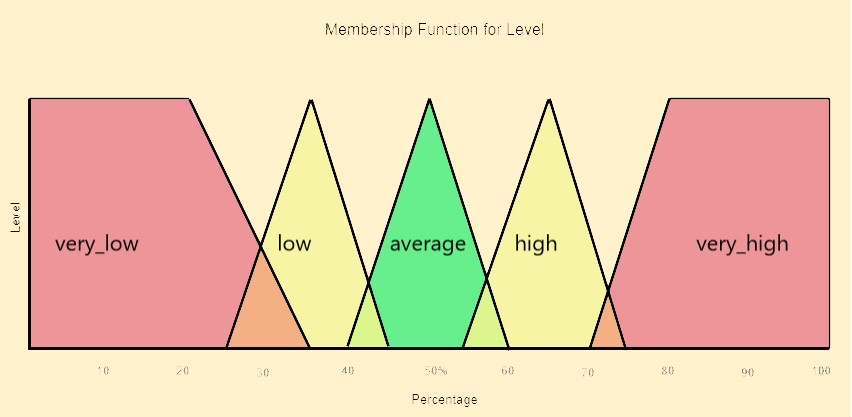
\includegraphics[keepaspectratio=true,scale=0.6]{__resources/level.jpg}
		\caption{Membership functions for Level}
		\label{member1}
	\end{center}
\end{figure}

\subsection*{Demand}
Like the level variable, five linguistic terms were made. The terms are as follows: \textbf{demand(d) = {very\_low, low, middle, high, very\_high}}. The demand variable has a range of -1 and 1.5. The same structure of two trapezoids and three triangle functions were used. 

\begin{figure}[ht]
	\begin{center}
		\advance\leftskip-3cm
		\advance\rightskip-3cm
		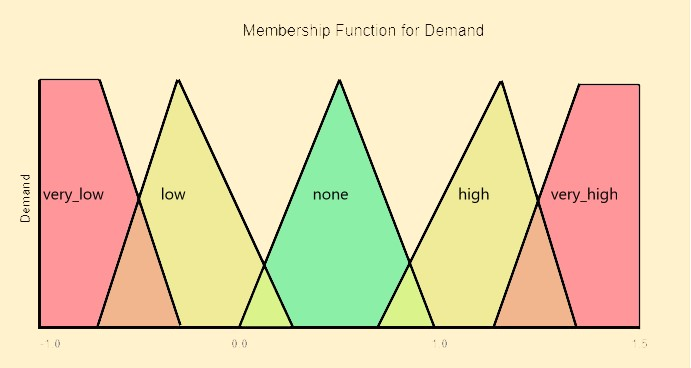
\includegraphics[keepaspectratio=true,scale=0.6]{__resources/demand.jpg}
		\caption{Membership functions for demand}
		\label{member2}
	\end{center}
\end{figure}


\newpage

\section*{Rule Terms}
in order to establish an output variable a set of rules must be defined control the value of the output variable. The three terms used for the output variable are as follows: \textbf{Command = {pump\_in, no\_pump, pump\_pump out}}. The following diagram shows the membership functions of the output variable command.
\begin{figure}[ht]
	\begin{center}
		\advance\leftskip-3cm
		\advance\rightskip-3cm
		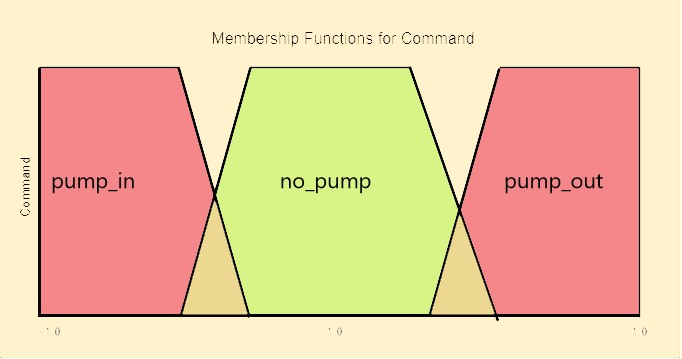
\includegraphics[keepaspectratio=true,scale=0.6]{__resources/command.jpg}
		\caption{Membership functions for command}
		\label{member2}
	\end{center}
\end{figure}
\newpage
A rule matrix will be utilized to illustrate the number of possible rules in the system. The top row signifies the demand variable with the terms it has been provided. Also, the first column displays the Level linguistic variable and it's terms. The intersection terms in the cells contain the command output variable that will be used to control the system.\\

\begin{tabular}{|c|c|c|c|c|c|}
	\hline 
	& \multicolumn{5}{c|}{\textbf{Demand}} \\ 
	\hline 
	\textbf{Level} & very\_low & low & middle & high & very\_high \\ 
	\hline 
	very\_low & pump\_in & pump\_in & pump\_in & pump\_in & no\_pump \\ 
	\hline 
	low & pump\_in & pump\_in & no\_pump & pump\_out & no\_pump \\ 
	\hline 
	average & no\_pump & no\_pump & no\_pump & pump\_out & pump\_out \\ 
	\hline 
	high & no\_pump & pump\_out & pump\_out & pump\_out & pump\_out \\ 
	\hline 
	very\_high & pump\_out & pump\_out & pump\_out & pump\_out & pump\_out \\ 
	\hline 
\end{tabular} \\\\
Following the implementation of the rule matrix, a set of some the possible rules that could be used in the system need to be defined using an \textit{IF-THEN} format. 


 \begin{longtable}{|l|>{\raggedleft\arraybackslash}p{4cm}|l|l|l}
	\hline 
 	\multicolumn{4}{|l|}{IF (level is very\_low) and (demand is very\_low or low or middle or high) THEN command is pump\_in} \\ 
 	\hline 
 	\multicolumn{4}{|l|}{IF (level is very\_low) and (demand is very\_high) THEN command is no\_pump} \\ 
 	\hline 
 	\multicolumn{4}{|l|}{IF (level is low) and (demand is very\_low or low) THEN command is pump\_in} \\ 
 	\hline 
 	\multicolumn{4}{|l|}{IF (level is low) and (demand is high or very\_high) THEN command is pump\_out} \\ 
 	\hline 
 	\multicolumn{4}{|l|}{IF (level is average) and (demand is very\_low or low or middle) THEN command is no\_pump} \\ 
 	\hline 
 	\multicolumn{4}{|l|}{IF (level is average) and (demand is high or very\_high) THEN command is pump\_out} \\ 
 	\hline 
 	\multicolumn{4}{|l|}{IF (level is high) and (demand is very\_low) THEN command is no\_pump} \\ 
 	\hline 
 	\multicolumn{4}{|l|}{IF (level is high) and (demand is low or middle or high or very\_high) THEN command is pump\_out} \\ 
 	\hline 
 	\multicolumn{4}{|l|}{IF (level is very\_high) and (demand is very\_low or low or middle THEN command is pump\_out} \\ 
 	\hline
 	\multicolumn{4}{|l|}{IF (level is very\_high) and (demand is high or very\_high) THEN command is pump\_out} \\ 
 	\hline 
 \end{longtable}

After some experimentation with the rules, it appeared that the more rules that were applied, and the more complex the rules were, the worse the system performed. Therefore, only five of the rules where kept in the final implementation. Using the check boxes, the controller maintains the level of water in the tank between the 40\% and 70\% requirement.



\section*{Conclusion}
In conclusion, this report laid out the purpose of this project, explained the linguistic variables and the terms used within those variable. Membership functions where illustrated for each variable and specified the rules used within the program to keep the controller at a state between the 40\% and 70\% requirements.  

\chapter{Methodology}


\section{section header 1}

\subsection{Subsection header 1}

\chapter{System Design}
//Brief introduction 

\section{Machine Learning Model}

\section{Data Preparation}

\section{Training}

\section{Deployment}

\section{System Architecture}
// insert topology here


\section{Concluding Analysis of System Design}

\chapter{Implementation}
The following chapter will outline the implementation process and how the project was developed. Firstly, an overview of the dataset used shall be given with information on how the images were preprocessed and augmented for training. A section for the model implementation will be given to describe how the convolutional neural network (CNN) was developed using Tensorflow. This is followed by the deployment process of the Tensorflow Python API. Lastly, the steps in which the Node.JS web application was made shall be touched upon, accompanied by the design and features choices.

\section{Data Understanding}
As stated in the system design, the dataset that will be used is the Cohn-Kanade+ image dataset, which release in 2000 with the purpose of classifying facial expressions \citep{ck}. The dataset consists of images of 210 subject between the ages of 18 and 50. Each subject is asked to show a a facial expression, beginning with a neutral facial expression that eventually lapses to the target emotion. The digital images come in either a 640x490 or 640x480 pixel format. Furthermore, the images either consists of an 8-bit grayscale or 24-bit colour format \citep{ck}. The dataset is made up of 593 image sequences and provides labels for each sequence, ranging between 0 and 6. Refer to Figure \ref{seq} for a summarized illustration of how these sequences are built.

\begin{figure}[ht]
	\begin{center}
		\advance\leftskip-3cm
		\advance\rightskip-3cm
		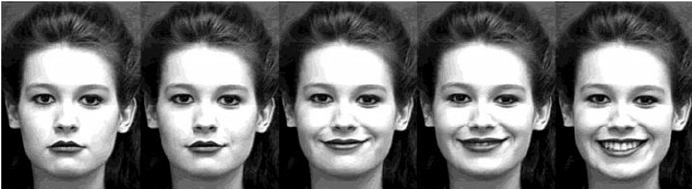
\includegraphics[keepaspectratio=true,scale=0.6]{__resources/DATASET/sequence.png}
		\caption{Image Sequence From Neutral to Happy}
		\label{seq}
	\end{center}
\end{figure}

It should be noted that the figure above is not a full image sequence and the some transitional images have been omitted. Moreover, it should also be known that there are inconsistencies in the dataset, such as a number subject not having image sequences for each certain emotions and label data missing for some images. This is acknowledged in the \textit{README} file created by Lucey et al. that is contained within the dataset, where it is declared "\textit{IF THERE IS NO FILE IT MEANS THAT THERE IS NO EMOTION LABEL (sorry to be explicit but this will avoid confusion)}". 

\section{Data Preparation and Preprocessing}
A number of preprocessing steps were taken in order to prepare the images for training the network. These steps were required to ensure maximum possible accuracy and minimal training time as the nature of working with neural networks can be computationally expensive when accompanied with large files such as images. The steps are as follows: Image extraction, Gray scaling, Facial Cropping, Data Augmentation and Data Splitting.

\subsection{Image Extraction}
Due to the structure of the image sequence within the datasets, it is undesirable to used all images within each sequence as that do accurately resemble the facial expression it is used to represent. Therefore, for each sequence the last four images were extracted from their directory and relocated to a new directory under the category of facial expression they represent. As stated in the system design, images for disgust and contempt are omitted from this new dataset. Furthermore, because there is now class for a neutral facial expression, the first four images from a sequence in each subject was extracted.

\subsection{Gray Scaling}
The CK+ dataset consist of a majority of gray images. However, the extended version of this dataset contains some images sequences with coloured images. When working neural networks, it is significantly more computationally expensive to process a coloured image over a gray one due to the number of colour channels. To mitigate this, a Python script was created to traverse through each image of the newly extracted dataset to convert all images to grayscale using the PILLOW library. \\

\begin{lstlisting}[language=Python, frame=single]
from PIL import Image
import numpy as np
import os, os.path
img_path = '<DATASET_DIRECTORY>' 

def grayify(file_name):
	image = Image.open(img_path + file_name)
	image = image.convert('L')
	image.save(img_path + file_name)

#Load the directory and traverse over all the image files
list = os.listdir(img_path)
for file in list:
	file_n = file
	print(file_n)

\end{lstlisting}

\subsection{Facial Cropping}
Following the gray scaling of all images, dimensionality reduction was implemented on the images. This was done by cropping each image down to only the facial surface area. This is done to reduce the noise of the data and to remove any features in the backgrounds that may be learned by the network that do not represent the facial expression. To do this, a Python script was written that reads in all the images from the dataset and crop the region of the image that contains the subject faces. This was done using the OpenCV library.

\begin{lstlisting}[language=Python, frame=single]
def facecrop(image):
	face_cascade = cv2.CascadeClassifier
	('haarcascade_frontalface_default.xml')
	
	img = cv2.imread(image)
	minisize = (img.shape[1],img.shape[0])
	miniframe = cv2.resize(img, minisize)
	faces = face_cascade.detectMultiScale(miniframe)
	
	for f in faces:
		x, y, w, h = [ v for v in f ]
		cv2.rectangle(img, (x,y), (x+w,y+h),
		(255,255,255))
		sub_face = img[y:y+h, x:x+w]
		fname, ext = os.path.splitext(image)
		cv2.imwrite(fname+"_cropped_"+ext, sub_face)
	return

list = os.listdir(<DIRECTORY_NAME>)
for file in list:
	facecrop(<DIRECTORY_NAME> + '/' + file)
\end{lstlisting}
\newpage
This was done for all images, however, some images were not correctly cropped due to noise in the image causing it to misclassify the facial region. Some examples of this might be only half the face being cropped into the new image or just the subjects shoulder being visible. These worthless images were manually deleted after the newly cropped images were evaluated. Please refer to Figure \ref{crop}for example of the facial cropping.

\begin{figure}[ht]
	\begin{center}
		\advance\leftskip-3cm
		\advance\rightskip-3cm
		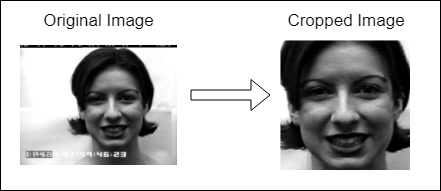
\includegraphics[keepaspectratio=true,scale=0.9]{__resources/DATASET/crop.png}
		\caption{Image Cropping on Facial Regions}
		\label{crop}
	\end{center}
\end{figure}
\newpage


\subsection{Image Increasing Through Data Augmentation}
Upon inspection of the dataset, in regards to the number of images for certain facial expressions, it was noted that there was an insufficient amount of images to train the network. This can be seen in table \ref{table: count}. 
\begin{table}
	\begin{tabular}{ |p{10cm}||p{3cm}|}
		\hline
		\textbf{Facial Expression} & \textbf{Cardinality}\\
		\hline
		\hline
		Anger & 601 \\
		\hline
		Fear & 427	\\
		\hline
		Happy & 883\\
		\hline
		Neutral & 668\\
		\hline
		Sad & 641	\\
		\hline
		Surprise  & 639	\\
		\hline
		\textbf{Total}  & \textbf{3879}	\\
		\hline
	\end{tabular}
	\caption{Initial Image Count}
	\label{table: count}
\end{table}

The initial step to increase the size of the data set was to flipped versions of all the images. Not only does this double the size of the dataset, but helps the network to better handle facial variance when dealing with new unseen data. Also, it will decrease the chance of under-fitting while training the model. Following this step, a check was done on the class balance. Using the Matplotlib Python library, the balance of each class was plotted by counting each image in accordance to it's respective label, as seen in Figure \ref{imbal}

\begin{figure}[ht]
	\begin{center}
		\advance\leftskip-3cm
		\advance\rightskip-3cm
		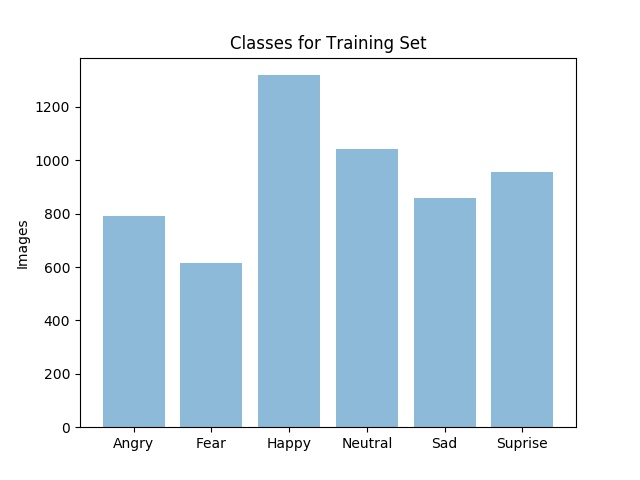
\includegraphics[keepaspectratio=true,scale=0.6]{__resources/implementation/imbalance.jpg}
		\caption{Class Imbalance}
		\label{imbal}
	\end{center}
\end{figure}\newpage
As seen above, expression 'Anger' and 'Fear' are under represented while 'Happy' is overly represented, relative to the rest of the dataset. How this problem was addressed was to create synthetic sample images from the existing ones by the means of skewing and augmenting the images. This can be seen in Figure \ref{augm}, where the top row displays the original cropped images. Beneath, are the slightly skewing images. This was implemented using a Python library called Augmentor, which allows you to specify the directory and number of altered samples you would like, and it randomly picks images within the directory, creating an entirely new back of images that have been stretched to a degree.
\begin{figure}[ht]
	\begin{center}
		\advance\leftskip-3cm
		\advance\rightskip-3cm
		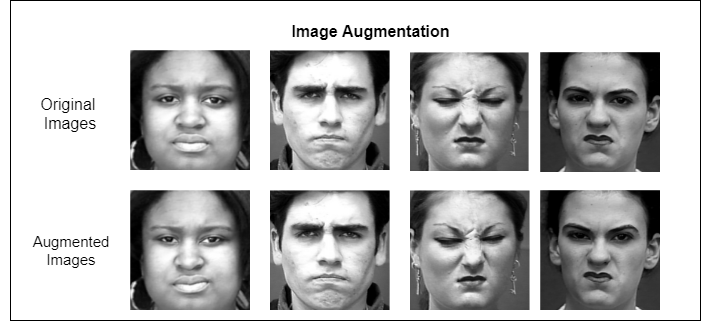
\includegraphics[keepaspectratio=true,scale=0.6]{__resources/implementation/augmented-images.png}
		\caption{Example of Augmented Images}
		\label{augm}
	\end{center}
\end{figure}
\newpage

This was done for all classes to increase the number of samples in the dataset, until a number of 1750 images are present for each class. This amounts to a total number of 10500 images in total across the entire dataset.  The class balance can be seen in the bar chart illustration in Figure \ref{bal}, which has been plotted using the Matplotlib library. In conclusion, an additional 6,621 images have been created from the original dataset.


\begin{figure}[ht]
	\begin{center}
		\advance\leftskip-3cm
		\advance\rightskip-3cm
		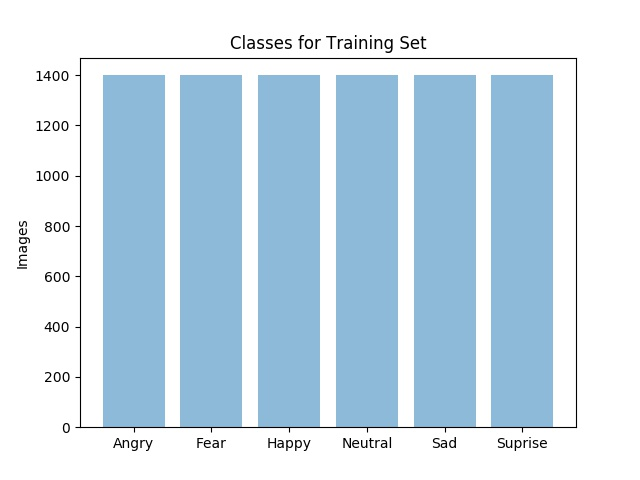
\includegraphics[keepaspectratio=true,scale=0.6]{__resources/implementation/balance.jpg}
		\caption{Class Balance}
		\label{bal}
	\end{center}
\end{figure}

\newpage

% show bad imbalance 
%flipping + synthethic examples
% show balance
\subsection{Data Splitting}
The last step in the the preparation phase was to apply split validation to the dataset. The dataset was split into training and testings sets at a divide of 80/20 - meaning 80\% of the dataset will be used for training (1400 images per class) and 20\% will be used for testing the model (350 images per class). Please see the Python code below showing how this was achieved.

\begin{lstlisting}[language=Python, frame=single]
import os, os.path
import math
from PIL import Image

old_path = 'C:/Users/aaron/Desktop/Cropped Dataset/happy/'

new_train_path ='C:/Users/aaron/Desktop/data/training/happy/'
new_test_path = 'C:/Users/aaron/Desktop/data/testing/happy/'

#Load the directory and traverse over all the image files
list = os.listdir(old_path)

# define the size of the first 80 percent of images
num_files = len(list)
num_training_files = num_files * .8
num_training_files = math.ceil(num_training_files)

num_testing_file = num_files * .2
num_testing_file = math.ceil(num_testing_file)

#Add the first 80 percent to the training folder
for img in list[1:num_training_files]: 
	i = Image.open(old_path + img)
	i.save(new_train_path+img)


#Add the remaining 20 percent to the training folder
for img in list[num_training_files:]:
	i = Image.open(old_path + img)
	i.save(new_test_path+img)
\end{lstlisting}

\section{Implementing the Machine Learning Model}

When implementing the machine learning model with Tensorflow, the initial step used is to import all the libraries that deemed necessary for preprocessing and training. These include Tensorflow, Numpy, Skimage, PIL etc. Secondly, the image data was import with it's respective labels. A list is used to store the image RGB data for every image in the dataset. Secondly, for each image in a directory under a certain class, a label of that class is added to the labels list. Refer code below to see how this was implemented.

\begin{lstlisting}[language=Python, frame=single]
def load_data(TRAINING_DIR):
images = []
labels = []

directories = [d for d in os.listdir(TRAINING_DIR) 
if os.path.isdir(os.path.join(TRAINING_DIR, d))]

# Traverse through each directory and make a list
# of files names if they end in the PNG format
for d in directories:
	label_directory = os.path.join(TRAINING_DIR, d)
	file_names = [os.path.join(label_directory, f) 
	for f in os.listdir(label_directory) 
				if f.endswith(".png")]
	
	#Traverse through each file, add the image data
	# and label to the 2 lists
	for f in file_names:
		images.append(skimage.data.imread(f))
		labels.append(int(d))
	return images, labels

images, labels = load_data(TRAINING_DIR)
\end{lstlisting}
Following this, shuffling of the data is performed, this is done to prevent overfitting of the model. Then further preprocessing steps are taken. In this case, each image in the list of images are sub sampled from their original sizes down to a 50x50 pixel size. This was done with the Skimage library to reduce the dimensionality of the images for the network to better handle the input data. The list images were traversed and resized using the tranform function. 
\begin{lstlisting}[frame=single]
images = [transform.resize(image,(50, 50))
	for image in images]
\end{lstlisting}
After basic data imports, defining the computation graph for Tensorflow is required. Tensorflow placeholder were then declared for later use when tensors need to be fed to the TensorFlow session, along with another few initial variables such as number of epochs, the batch size, dropout rate etc. When all the main variables needed for TensorFlow are made, the structure of the network was mad. This was done using the tf.slim library, which a TensorFlow package that allows you to define layers in a network easily. 

In total there are 10 convolution layers with 5 MaxPooling layers. The convolution layer is used to extract features within the image while pooling reduces the dimensionality of the feature maps, but retains majority of the useful data.
\begin{figure}[ht]
	\begin{center}
		\advance\leftskip-3cm
		\advance\rightskip-3cm
		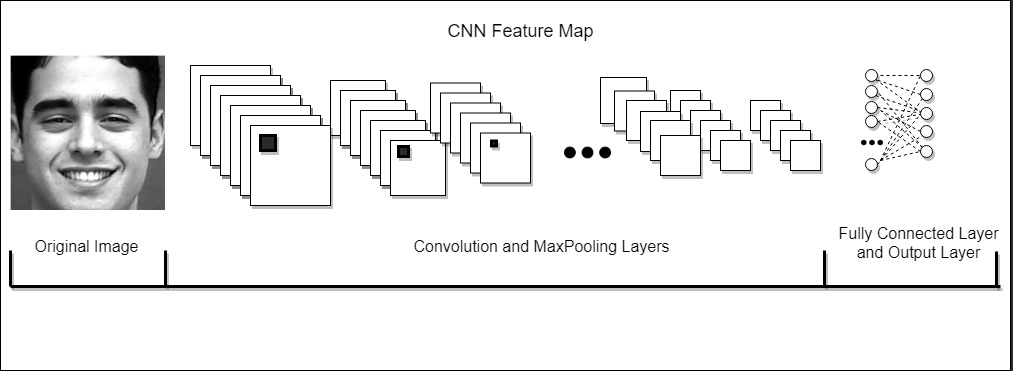
\includegraphics[keepaspectratio=true,scale=0.5]{__resources/implementation/map.jpg}
		\caption{Feature Map of CNN}
		\label{map}
	\end{center}
\end{figure}
Lastly, a fully connected layer is defined, which will be used to produce a predicted output.The reason dropout is used in this case is to reduce the chances of over fitting the network. After each training iteration (epoch), only 80 percent of the trained neurons are kept.\\ \\



\begin{lstlisting}[language=python, frame=single]
	net = slim.conv2d(net, 32, 3)
	net = slim.conv2d(net, 64, 3)
	net = slim.conv2d(net, 64, 3)
	net = slim.max_pool2d(net, 3, stride = 1 )
	net = slim.conv2d(net, 96, 3)
	net = slim.conv2d(net, 96, 3)
	net = slim.max_pool2d( net, 2, stride = 2)
	
	net = slim.conv2d(net, 128, 3)
	net = slim.conv2d(net, 128, 3)
	net = slim.max_pool2d( net, 2, stride = 2)
	
	net = slim.conv2d(net, 128, 3)
	net = slim.conv2d(net, 128, 3)
	net = slim.max_pool2d(net, 2, stride = 2)
	
	net = slim.conv2d(net, 128, 3)
	net = slim.max_pool2d(net, 2, stride = 1)
	
	net = slim.dropout(net, keep_prob = keep_rate
		, is_training = is_training )
\end{lstlisting}

Following the structure set up of the network, a function is defined that runs the Tensorflow session, which takes the \textbf{x} placeholder as a parameter.
Within this function we define the loss function used within the network which is softmax with cross entropy. Also the Adam optimizer is used for back propagating through the network and adjusting the weights. A learning rate of 0.002 was chosen for the final implementation after showing in experimentation that this reduced the loss the most. 

\begin{lstlisting}[language=python, frame=single]
loss = tf.reduce_mean(tf.nn.softmax_cross_entropy_with_logits
    (labels = y, logits = output))
total_losses = tf.losses.get_total_loss
	( add_regularization_losses=True ) + loss

update_ops = tf.get_collection(tf.GraphKeys.UPDATE_OPS)
with tf.control_dependencies(update_ops):
train_op = tf.train.AdamOptimizer( learning_rate=0.002 )
			.minimize( total_losses )
\end{lstlisting}


When the session is ran, the TensorFlow variables are initialized and the training begins. 
The list of images and labels are segmented into batches of size 100 to prevent an OOM error, as loading all the images into memory can cause an overflow. The images and labels are fed into the TensorFlow runtime environment for training. After each epoch, the accumulated loss and batch accuracy is calculated and printed to the screen.
After the network have been trained for the specified number of epochs, it evaluated the accuracy on the test data and a TensorFlow \textit{.CKPT} model file is saved to disk.

% Image images
% preprocessing
% Create comptation graph
% create session

\section{Deploying the Trained Model}
% 1 - Flask API

/***********************************/

\section{Implementing the Node.JS Application}
To develop a web application for the user to interact with, Node.JS was used to implement a simple one page application that accesses the users webcam. Firstly, a javascript webserver was created using the Express npm module, which provides functions for routing and serving html pages. A port is initially set using either port 5000 for local development, or a randomly allocated port for deployment. 

\begin{lstlisting}[language=python, frame=single]
	app.set('port', (process.env.PORT || 5000))
\end{lstlisting}

This is followed by providing the home page when the base route is called by from the client. When the \textbf{'/'} route is called, a html page containing the application is delivered to the users browser and displayed in the DOM.

\begin{lstlisting}[language=python, frame=single]
app.get('/', function (req, res) {
  res.sendFile(path.join(__dirname, '/index.html'));
});

var server = app.listen(app.get('port'), function () {
  var host = server.address().address
  console.log('Application running on port', app.get('port'))
})
\end{lstlisting}

\subsection{Facial Tracking With a Users Webcam}

The user interface design of the application is very simple. On the left hand side a the page the webcam feed is displayed. This accesses the user's machine's webcam and displays it to the screen using the html \textbf{canvas} element. Canvas is a container for drawing graphics to the page. For facial tracking, a library called Tracking.js was imported. Trackin.js is an open source library created by Eduardo Lundgren for object, colour and face detection using javascript. The reason for this library choice was because other alternatives, such as OpenCV, deemed to be very heavy weight in comparison and API services that have also been considered such as cloudinary would reduce classification speed as it would be computationally expressive to make multiple requests for facial cropping while using the application. 
In light of this, tracking.js provides a lightweight and quick solution for detecting faces. Using what is known as haar cascades, object classification and detection is made simplified and provides fast calculation speeds. In terms of the web application, the canvas drawing of the webcam feed is read and interpreted by tracking.js and the facial features are detected. A yellow box is drawn around the detected facial area.
\begin{lstlisting}[language=python, frame=single]
var tracker = new tracking.ObjectTracker('face');
tracker.setInitialScale(4);
tracker.setStepSize(.5);
tracker.setEdgesDensity(0.1);
tracking.track('#video', tracker, { camera: true });
tracker.on('track', function(event) {
context.clearRect(0, 0, canvas.width, canvas.height);
\end{lstlisting}

One function that tracking.js does not provide is the ability to crop the detected area of the stream. To get around this, java script code was developed to mark the area in which the square was being drawn around the users face. In each frame of a users face being detected a new square is drawn to the canvas, so every time that a new square is displayed to the screen, this marks the new coordinates of the area in which is needed for cropping. 

\begin{lstlisting}[language=python, frame=single]
rect_width = rect.width; // 
rect_height = rect.height;
rectX = rect.x;
rectY = rect.y;

 ...

ctx.drawImage(video, rectX+ 100, rectY +90,
	 rect_width +70,  rect_height +50, 0, 0, 300, 150);
\end{lstlisting}

After is is known where the users face is positioned in the shot, the cropped area is displayed in a separate 100x100 pixel canvas area, named ctx, below the feed. To ensure that the trained Tensorflow API does not become overflowed with image data, an interval timing is implemented. This involves setting a timer as to when an image is cropped because it would be disadvantageous and computationally expensive to have every frame to be sent to the API. In this case, the interval is set to 1 second. To initiate a session with the model and begin the facial sentiment analysis, a button was added to the UI which begins the analysis. Please refer to the Figure \ref{web} for a screenshot of the facial tracking in action.

\begin{figure}[ht]
	\begin{center}
		\advance\leftskip-3cm
		\advance\rightskip-3cm
		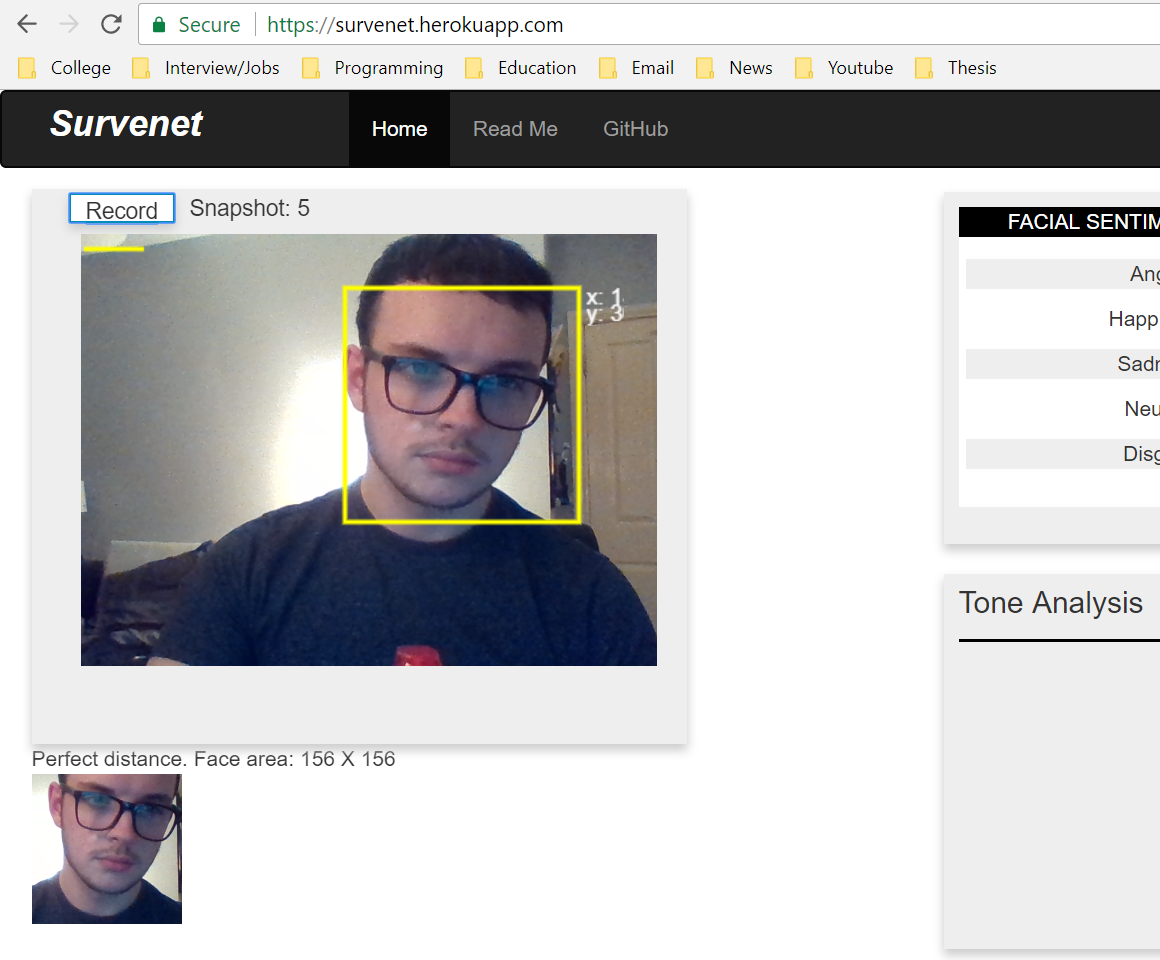
\includegraphics[keepaspectratio=true,scale=0.5]{__resources/implementation/webapp1.png}
		\caption{Webcam Feed with Facial Tracking and Cropping}
		\label{web}
	\end{center}
\end{figure}

\newpage

%\subsection{Facial Sentiment Analysis} 

% 1 - Create Node/express application
% 2 - Implement webcam canvas
% 3 - Apply tracking.js
% 4 - impelement facial cropping
% 5 - Make request to API

\section{Deploying the Node.JS Application}
% 1 - Github
% 2 - Heroku integration

For deploying the web application, the Heroku PaaS of service was used. Using GitHub integrations, whenever a new version of the application was pushed to the remote repository a new build was commenced. If the build was successful, the application would be live for use at \textit{https://survenet.herokuapp.com}.

%\subsection{Database Integration
%\section{Result Weighting Algorithm}
%\section{Integrating Third Party Services}
\section{Concluding Remarks of Implementation}

In summary, many data preprocessing steps were taken to ensure the best possible result of the model. These include gray scaling, facial cropping, data increase by creating flipped copies and image augmentation. These steps were taken to ensure the best possible results when evaluating the model. Secondly, the data was split into training and testing sets. A fully working TensorFlow model was created in python and trained on the FloydHub could training platform. A facial tracking web application was built for recording the used face and deployed to the heroku PaaS. 




\prefacesection{Expected Results}


\section*{section header 1}

\subsection*{Subsection header 1}


\chapter{Results and Discussion}


\section{section header 1}

\subsection{Subsection header 1}

% \prefacesection{Project plan}




\setlinespacing{1.0}
\bibliographystyle{plainnat}
\bibliography{bibliography}

\prefacesection{Project plan}




\end{document}
% ------------------------------------------------------------------------
%%%      \setlength\LTleft{1pt}
